\chapter{Experimentación y Análisis de Resultados}
\label{chap:experimentacion}

Una vez descritos los fundamentos teóricos de Word2Vec y QWord2Vec, este capítulo recoge el proceso de experimentación llevado a cabo para comparar ambos modelos. Se han desarrollado las implementaciones de ambos algoritmos en el lenguaje de programación \textit{Python}.

Para el modelo clásico, se ha empleado la implementación disponible en la librería \textit{Gensim}, que incluye tanto la arquitectura del modelo como la función de optimización Negative Sampling, desarrollada siguiendo las especificaciones originales de Google. Por su parte, la versión cuántica ha sido implementada utilizando la librería \textit{Qiskit}, que proporciona las herramientas necesarias para la construcción del circuito parametrizado, la aplicación del optimizador descrito en el capítulo anterior, así como utilidades para la medición y transpilación del circuito.

El objetivo principal de esta experimentación es evaluar si los \textit{embeddings} generados por QWord2Vec son capaces de preservar relaciones semánticas entre palabras de forma comparable a los producidos por Word2Vec. Para ello, se ha seguido una metodología sistemática que abarca desde la preparación del corpus y la configuración de los hiperparámetros, hasta el análisis de la función de pérdida durante el entrenamiento y la evaluación de la calidad de los \textit{embeddings} mediante el coeficiente de correlación de Pearson. Asimismo, se incluye un análisis comparativo de los tiempos de ejecución de ambos modelos, dado que el coste computacional es uno de los factores críticos en el contexto de la computación cuántica simulada.

\section{Metodología experimental}

Esta sección describe los pasos previos necesarios para llevar a cabo la experimentación. En primer lugar, se presenta el corpus empleado para el entrenamiento de ambos modelos, junto con el proceso de preprocesamiento aplicado en cada caso. A continuación, se detallan las herramientas y el entorno de ejecución utilizados, aspecto especialmente relevante en el caso de QWord2Vec, dado que la simulación clásica de circuitos cuánticos impone restricciones significativas sobre el tamaño del experimento realizable.

\subsection{Dataset y preprocesamiento}

Como se comentó anteriormente, la simulación clásica de circuitos cuánticos impone restricciones severas sobre el tamaño del experimento. A diferencia de Word2Vec clásico, que habitualmente se entrena con corpus de millones de frases y vocabularios de cientos de miles de palabras, el coste computacional de simular un circuito cuántico crece exponencialmente con el número de qubits, lo que hace inviable trabajar con corpus de gran escala en un entorno de computación personal que es con el que se ha trabajado.

Por este motivo, se ha adoptado el mismo corpus empleado en el trabajo de referencia \cite{ohno_qword2vec_2025}, el cual fue tomado originalmente de una fuente web la cual ofrecía corpus pequeños para realizar evaluaciones de modelos de este estilo, solo que actualmente no está disponible la página web. El corpus consta de 13 frases en inglés con un vocabulario de 13 palabras únicas. Las frases utilizadas son las siguientes:

\begin{quote}
  \ttfamily
  i like dog \quad i like cat \quad i like animal \quad dog cat animal \\
  apple cat dog like \quad dog fish milk like \quad dog cat eyes like \\
  i like apple \quad apple i hate \quad apple i movie \\
  book music like \quad cat dog hate \quad cat dog like
\end{quote}

Las frases tienen una longitud de entre 3 y 4 palabras, lo que condiciona el tamaño de la ventana de contexto haciendo que sea pequeña. Desde el punto de vista de la distribución léxica, el corpus presenta un desequilibrio: las cuatro palabras más frecuentes (\textit{like}, \textit{dog}, \textit{cat} e \textit{i}) concentran el 67\% de los tokens totales, mientras que seis palabras del vocabulario aparecen una única vez. Este desequilibrio puede introducir distorsiones en las relaciones semánticas aprendidas por el modelo, y es una limitación que se asume de forma consciente.

No obstante, el uso de este corpus está justificado por tres razones. En primer lugar, permite reproducir directamente las condiciones experimentales del paper de referencia, facilitando la comparación de resultados durante el desarrollo e implementación de variaciones que se han realizado. En segundo lugar, el objetivo del estudio no es obtener un modelo de procesamiento del lenguaje natural de calidad, sino evaluar si QWord2Vec es capaz de preservar las relaciones semánticas que aprende Word2Vec. Para este fin, un corpus pequeño y controlado es suficiente. En tercer lugar, el tamaño reducido del vocabulario permite inspeccionar e interpretar los \textit{embeddings} obtenidos de forma directa, verificando manualmente que las relaciones semánticas resultantes son coherentes con el contenido del corpus.

En cuanto al preprocesamiento, no se ha realizado nada ya que el corpus viene preprocesado con sus palabras separadas por un espacio tal y como se espera sin necesidad de haber tenido que eliminar algún signo de puntuación o bien convertir todo a minúscula.

\subsection{Entorno de ejecución y herramientas}

Todos los experimentos se han llevado a cabo sobre un ordenador personal con sistema operativo Ubuntu, cuya compatibilidad con las librerías empleadas y su integración con el hardware disponible lo hacen especialmente adecuado para este tipo de desarrollo. Las características del hardware relevantes para el rendimiento son las siguientes:

\begin{itemize}
  \item \textbf{Procesador}: Intel Core i7-13700F (30\,MB de caché, frecuencia máxima superior a 5,2\,GHz).
  \item \textbf{Memoria RAM}: 32\,GB DDR4 a 3600\,MHz.
  \item \textbf{Tarjeta gráfica}: MSI GeForce RTX 4070 con 12\,GB de memoria GDDR6X.
\end{itemize}

En cuanto al software, las librerías principales utilizadas en el desarrollo son:

\begin{itemize}
  \item \textbf{Python} 3.10.12: lenguaje de programación base del proyecto.
  \item \textbf{Gensim} 4.4.0: empleada para la implementación del modelo Word2Vec clásico.
  \item \textbf{Qiskit} 1.4.5: utilizada para la construcción y ejecución del circuito cuántico parametrizado.
  \item \textbf{Qiskit Aer} 0.17.2: backend de simulación cuántica sobre hardware clásico.
\end{itemize}

Respecto a la elección del simulador cuántico, \textit{Qiskit} ofrece tres opciones: \textit{AerSimulator}, \textit{StatevectorSimulator} y \textit{QasmSimulator}. Los dos últimos se encuentran en proceso de deprecación, dado que \textit{AerSimulator} los unifica y supera en capacidades siendo el que más soporte y desarrollo recibe. Por este motivo, se ha optado por \textit{AerSimulator} como backend de simulación para la ejecución de QWord2Vec.

\section{Configuración de hiperparámetros}

Tanto el modelo clásico como el cuántico presentan una serie de hiperparámetros que deben ajustarse para obtener el mejor rendimiento posible, como ocurre en cualquier problema de \gls{ml}. Para su configuración se ha empleado la técnica de búsqueda exhaustiva \textit{Grid Search}, implementada manualmente en ambos casos al no disponer de una implementación genérica compatible con los modelos utilizados.

La estrategia seguida ha consistido en identificar, a partir de la literatura y de experiencias previas en problemas similares que han comentado distintas personas en foros, un conjunto de valores de referencia para cada hiperparámetro. A partir de estos valores, se han definido rangos de búsqueda que incluyen el valor de referencia junto con variaciones por encima y por debajo, con el objetivo de ajustar cada parámetro al corpus y al problema concreto. Dado que ambos modelos emplean funciones de pérdida y algoritmos de optimización distintos, cada uno dispone de su propio conjunto de hiperparámetros a explorar.

\subsection{Hiperparámetros de Word2Vec}

Los hiperparámetros de Word2Vec pueden agruparse en tres categorías según el componente del modelo al que pertenecen: los propios de la arquitectura Skip-Gram, los relacionados con Negative Sampling y el correspondiente al optimizador.

En cuanto a los hiperparámetros de \textbf{Skip-Gram}, los dos parámetros ajustados son \textit{vector\_size} y \textit{window}. El primero determina la dimensionalidad de los vectores de \textit{embedding}, es decir, el número de características con el que se representa cada palabra. Su elección depende del tamaño del vocabulario, la riqueza semántica del corpus y los recursos computacionales disponibles. Dado que el vocabulario es de únicamente 13 palabras, no se requiere una representación de alta dimensionalidad para capturar las relaciones semánticas presentes. Por ello, se exploraron valores en el rango $\{2, 3, 4\}$. El valor seleccionado por el \textit{Grid Search} fue $\text{vector\_size} = 2$, lo cual resulta coherente con el reducido tamaño del vocabulario y presenta la ventaja adicional de permitir visualizar directamente los \textit{embeddings} en el plano y realizar una validación manual sin necesidad de aplicar técnicas de reducción de dimensionalidad como PCA.

El segundo parámetro, \textit{window}, define la distancia máxima entre la palabra central y las palabras de contexto consideradas durante el entrenamiento, tal y como se ilustra en la Figura \ref{fig:window_ilustracion}. Los valores explorados fueron $\{1, 2, 3\}$, teniendo en cuenta que las frases del corpus tienen entre 3 y 4 palabras: con una ventana de tamaño 2, la palabra central puede relacionarse con todas las demás en una frase de 4 palabras, mientras que con tamaño 1, solo se considera la palabra adyacente. El valor seleccionado fue $\text{window} = 1$, lo que implica que el modelo aprende exclusivamente a partir de pares de palabras contiguas, una restricción adecuada dada la brevedad de las frases del corpus.

\begin{figure}[h]
  \centering
  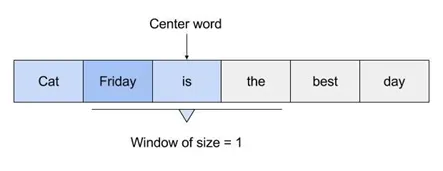
\includegraphics[width=0.7\linewidth]{imagenes/windowIlustration.png}
  \caption{Ilustración del parámetro \textit{window} en Skip-Gram: distancia máxima desde la palabra central hasta las palabras de contexto consideradas. Fuente: \url{https://medium.com/@zafaralibagh6/a-simple-word2vec-tutorial-61e64e38a6a1}.}
  \label{fig:window_ilustracion}
\end{figure}

Respecto a los hiperparámetros de \textbf{Negative Sampling}, los parámetros explorados son \textit{negative} y \textit{ns\_exponent}. El primero indica el número de muestras negativas que se generan por cada par positivo durante el entrenamiento. El paper original que publicó Google, recomendó valores entre 5 y 20 (siendo 20 para corpus de gran escala). Dado que el corpus empleado cuenta únicamente con 13 palabras únicas, se optó por explorar valores en el rango $\{2, 3, 5, 6\}$, descartando valores superiores a la mitad del vocabulario para evitar que Negative Sampling degenerase en un comportamiento equivalente al softmax completo sobre todo el vocabulario, además de tener en consideración la recomendación del paper de Google. El valor seleccionado fue $\text{negative} = 5$, coincidiendo con el mínimo recomendado en el paper original.

El parámetro \textit{ns\_exponent} controla la distribución de probabilidad con la que se seleccionan las palabras negativas. Un valor de 1 desfavorece a las palabras poco frecuentes respecto a una distribución puramente proporcional a las frecuencias, mientras que un valor de 0,0 trata todas las palabras con igual probabilidad. El paper original de Word2Vec estableció 0,75 como valor fijo, sin embargo, un estudio posterior \cite{caselles_word2vec_hyperparameters_2018} argumentó que este parámetro debería adaptarse al problema concreto. Dado el notable desequilibrio léxico del corpus utilizado, se exploraron los valores $\{0{,}0,\ 0{,}3,\ 0{,}75\}$. El valor seleccionado fue $\text{ns\_exponent} = 0{,}0$, lo que implica que todas las palabras tienen igual probabilidad de ser seleccionadas como muestras negativas, compensando en parte el desequilibrio de frecuencias del corpus.

Por último, el hiperparámetro relacionado con el \textbf{optimizador} es \textit{alpha}, que establece la tasa de aprendizaje inicial del modelo. \textit{Gensim} gestiona internamente la evolución de esta tasa a lo largo del entrenamiento, permitiendo únicamente fijar su valor inicial. La búsqueda de este parámetro se realizó en dos fases iterativas. En una primera exploración se consideró el rango $\{0{,}1,\ 0{,}15,\ 0{,}175,\ 0{,}2\}$, con el objetivo de comprobar si valores pequeños eran suficientes para la convergencia. El valor seleccionado en esta fase fue $0{,}2$, el límite superior del rango, lo que indicó que el modelo requería tasas de aprendizaje más elevadas. A partir de este resultado, se acotó el rango de búsqueda hacia valores superiores, explorando $\{0{,}2,\ 0{,}25,\ 0{,}275,\ 0{,}3\}$. En esta segunda fase el valor seleccionado fue $\text{alpha} = 0{,}25$, situándose en el interior del rango y confirmando que la convergencia óptima se alcanza con tasas de aprendizaje relativamente elevadas.


\subsection{Hiperparámetros de QWord2Vec}

En cuanto a los hiperparámetros de la parte cuántica, se puede dividir en 3 bloques principales que son: Hiperparámetros del circuito, hiperparámetros relacionados con \gls{qng} y los hiperparámetros relacionados con \gls{spsa}. Estos 2 últimos, en la clase utilizada la cual tiene el algoritmo \gls{qn-spsa} implementado, contiene los hiperparámetros relacionados a \gls{qng} y los relacionados a \gls{spsa} para juntarlos en el algoritmo que los engloba.

En cuanto a los hiperparámetros del circuito, solo se puede tener en cuenta el número de iteraciones que realiza así como el número de muestras que toma en una simulación. Para el primer hiperparámetro, se ha tenido en cuenta que los circuitos variacionales cuánticos suelen necesitar muchas épocas para converger. El paper principal en el que se ha basado para implementar este circuito cuántico \cite{ohno_qword2vec_2025}, utilizó para su circuito un máximo de 30.000 épocas (utilizando otra función de optimización menos eficiente que la que se ha propuesto aquí). Por lo que teniendo en cuenta el número de épocas tan grande pero que también la función de optimización \gls{qn-spsa} está diseñada para que converga con pocas épocas, decidí utilizar 1500 iteraciones como máximo. En cuanto al número de muestras obtenidas en cada simulación, seleccioné una gran cantidad para tener una distribución de valores más limpia y exigente, siendo así los resultados lo más honesto posibles evitando que haya mucha varianza estadística, por ello utilicé 1024 shots por cada simulación. Otro hiperparámetro a configurar, fue el valor \textit{A\_{th}} que se utiliza en la fórmula del cálculo heurístico de número de capas, este parámetro viene a indicar cuál es el límite superior de datos de entrenamiento que se está dispuesto a perder. Para establecer este valor, se ha tenido en cuenta que en el paper el cual indicaba la heurística para calcular la longitud del circuito, indicaba que los mejores parámetros de \textit{A\_{th}} que le funcionó, estaban entre 0.01 y 0.05. Por ello en el gird search primero se probó con valores muy dispares de 0.01, 0.03 y 0.05 y viendo que se quedó con el 0.03 luego se probó valores algo superiores e inferiores a 0.03 encontrando así que el mejor Ath posible para el corpus que se tiene y el resto de hiperparámetros calculados ha sido 0.21.

Para los hiperparámetros de SPSA, en concreto los que gestiona cómo va decayendo la tasa de aprendizaje y la perturbación, se ha utilizado las fórmulas que indica el autor en su paper original de este algoritmo \cite{spall_spsa_1998}. De estas fórmulas, hay 4 valores posibles a ajustar, que son: los 2 coeficientes de cuanto decaimiento tienen los valores de la tasa de aprendizaje y de perturbación a lo largo de las épocas y luego los otros 2 coeficientes iniciales del leraning rate y perturbación. Pues bien, de estos 4 posibles valores, solo se han fine tuneado los 2 últimos. Esto se ha decidido así porque como bien indica en el paper, los valores de decaimiento que propone ya han sido probados matemáticamente y empíricamente por lo que son los valores recomendables a utilizar mientras que los valores de la tasa de aprendizaje inicial así como de la perturbación son valores que se tienen que ajustar a cada tipo de problema. Teniendo eso en cuenta, se probó con valores bajos de learning rates y de perturbaciones sabiendo que se aplicaba un educated guess al inicio. Un educated guess significa que en vez de elegir valores aleatorios de pesos, se prueba de manera aleatoria durante un cierto número de iteraciones de y se queda con aquellos pesos que hayan dado mejores resultados en las simulaciones. En este caso el educated guess ha sido de 10 iteraciones por cada parámetro. Teniendo en cuenta esta pequeña técnica aplicada para mejorar los pesos iniciales, fue uno de los motivos principales por los que no se quiso usar un learning rate alto, es decir, ya se tendrían unos hiperparámetros que podrían ir en buena dirección. <cuando corrigas esto Claude, méteme algún argumento mejor o algo de por qué usar valores pequeños para los hiperaprámetros de inicio de learning rate y de perturbación>

Además se decidió establecer el parámetro \textit{blocking} a true para que así el optimizador solo aceptara mejoras de un valor de pérdida no más grande que el anterior actualizado añadido con una tolerancia.

El resto de parámetros a configurar, ha sido todo lo relacionado con el \gls{qng}, al principio he buscado en la literatura clásica que venía explicada \cite{duan_qnspsa_pennylane_2022} cuáles eran los hiperparámetros que se debían de ajustar. De ahí se siguió las recomendaciones de configurar el tensor métrico de Fubiny-Study como la matriz identidad en $g^{(0)}$. También se tomó en consideración buscar el mejor valor del hiperparámetro del coeficiente de regularización, así cuando se aplicara el valor del tensor métrico de Fubiny-Study cerca de un mínimo, no se desvaneciera dicho tensor. De este hiperparámetro se tuvo en cuenta las consideraciones de no tomar un valor muy alto ya que eliminaría toda la información del tensor mético de Fubiny-Study pero un valor muy bajo haría que se desvaneciera en el límite. Además para validar si sería necesario utilizar esta función de optimización ya que es muy compleja además de que tiene mucha potencia, se ha decidido establecer otro hiperparámetro que es el \textit{Hessian Delay}, este hiperparámetro controla cuando se debe de aplicar el tensor métrico de Fubiny-Study. Esto se ha decidido establecer ya que al principio con mucho ruido puede hacer que no se comporte bien del todo. Además se ha establecido otro hiperparámetro que es el resampling. Esto indica cuántas veces se tiene que ejecutar el cálculo del tensor métrico de Fubiny-Study y hacer una media de los valores obtenidos. Se ha puesto un resampling bajo ya que este introduce una mayor sobrecarga a lo dificultoso que es de ejecutar el algoritmo de por si. Se ha establecido este hiperparámetro con el objetivo de ver si es necesaria tanta complejidad en la función de optimización para este problema, o bien utilizando solo el SPSA al igual que hace el paper original pero con unos mejores hiperparámetros, daba mejores resultados. Otro hiperparámetro que ha habido que establecer es la fidelidad, para calcular este tensor a nivel práctico se tiene que hacer sobre el circuito que se quiere optimizar. En este caso al ser un corpus de 13 palabras, se tienen 13 circuitos distintos ya que cada uno tiene su codificación de manera independiente en el espacio de Hilbert. Por lo que para no calcular siempre el tensor métrico de Fubiny-Study sobre el mismo circuito, se ha ido rotando de manera uniforme para que calculara el valor con distintos circuitos y así evitar que solo afectara a una palabra perjudicando a todas las demas palabras utilizadas.

\section{Entrenamiento}

En esta sección se describe el proceso de entrenamiento seguido para cada modelo. Dado que Word2Vec y QWord2Vec emplean funciones de pérdida y algoritmos de optimización distintos, el análisis de cada uno se presenta de forma independiente.

\subsection{Word2Vec}

El proceso de entrenamiento de Word2Vec se basa en la función de pérdida de Negative Sampling como se explicó con anterioridad. Sin embargo, minimizar esta función auxiliar no garantiza directamente una buena calidad semántica de los \textit{embeddings}. Por ello, se ha incorporado una métrica de evaluación adicional basada en el algoritmo \textit{K-Means}, que permite cuantificar de forma directa la coherencia semántica de los vectores obtenidos.

El rol de cada componente es el siguiente. \textbf{Train loss} actúa como función de optimización, proporcionando la señal con la que el optimizador actualiza los parámetros en cada iteración. El \textbf{K-Means accuracy} constituye la métrica de calidad real de los \textit{embeddings} y es la que determina el criterio de parada. Esta distinción es importante, usar el loss como criterio de \textit{Early Stopping} podría interrumpir el entrenamiento en un punto subóptimo desde el punto de vista semántico, ya que el loss de Negative Sampling puede seguir oscilando incluso cuando los \textit{embeddings} han convergido a su mejor configuración.

Para calcular la precisión de \textit{K-Means}, es necesario disponer de un agrupamiento (también conocido como clusters) de referencia (\textit{ground truth}) de las palabras del vocabulario. Dicho agrupamiento fue generado mediante el modelo de lenguaje Gemini 3.0 Pro a partir del corpus, con la restricción de que los grupos fueran lo más equilibrados posible y sin poder aparecer la misma palabra en distintos grupos. El resultado fue posteriormente validado manualmente, obteniéndose los siguientes cuatro clústeres:

\begin{itemize}
  \item \textbf{animal}: \textit{dog, cat, animal, eyes}
  \item \textbf{food}: \textit{apple, fish, milk}
  \item \textbf{culture}: \textit{book, music, movie}
  \item \textbf{sentiment}: \textit{i, like, hate}
\end{itemize}

Dado que \textit{K-Means} asigna etiquetas arbitrarias a los clústeres, la precisión se calcula mediante el algoritmo húngaro, que encuentra la correspondencia óptima entre los clústeres predichos y los de referencia antes de evaluar el porcentaje de palabras correctamente asignadas.

Esta evaluación no se realiza en cada época, sino cada 200 épocas de entrenamiento. Esta frecuencia permite que el modelo evolucione suficientemente entre comprobaciones, manteniendo un equilibrio entre la sensibilidad de la métrica y la carga computacional adicional que supone ejecutar \textit{K-Means} sobre los \textit{embeddings} actuales.

La técnica de \textit{Early Stopping} monitoriza el K-Means accuracy en cada comprobación y detiene el entrenamiento si no se supera el mejor valor previo en al menos un delta mínimo de 0,01 durante 5 comprobaciones consecutivas (paciencia = 5). En ese punto se recupera los pesos de los parámetros correspondiente al mejor accuracy registrado, reduciendo el riesgo de sobreajuste y garantizando que el modelo devuelto es el que mejor agrupa semánticamente las palabras.

Respecto a la partición de los datos, el entrenamiento se ha realizado con el 100\% del corpus, sin reservar un conjunto de validación o prueba. Esta decisión fue tomada ya que uno de los objetivos del experimento de la versión clásica no es evaluar la capacidad de generalización del modelo a palabras nuevas, sino obtener \textit{embeddings} de referencia para todas las palabras del vocabulario. Dado que Word2Vec solo genera un vector para una palabra si la ha observado durante el entrenamiento, excluir un subconjunto de frases implicaría que algunas palabras del vocabulario carecerían de embedding, dificultando la comparación con QWord2Vec, que requiere los vectores de referencia de todo el corpus.

En cuanto al flujo de entrenamiento, las frases del corpus se reordenan aleatoriamente antes del entrenamiento para evitar que el modelo aprenda varias frases consecutivas cuyos valores están definidos en el mismo clúster, favoreciendo una exploración más amplia del espacio de parámetros. Se utiliza una semilla fija (valor 42) para garantizar la reproducibilidad de los resultados. El modelo se entrena desde cero utilizando los mejores hiperparámetros encontrados en el \textit{Grid Search}. Una vez finalizado el entrenamiento, los \textit{embeddings} de la mejor época encontrada, se exportan a un fichero de texto plano para su uso como referencia de comparación en la implementación cuántica.

La evolución del K-Means accuracy y del train loss delta a lo largo del entrenamiento se puede observar en la Figura \ref{fig:loss_curves_word2vec}.

\begin{figure}[h]
  \centering
  
\includegraphics[width=0.85\linewidth]{imagenes/lossCurvesWord2Vec.png}
  \caption{Evolución del K-Means accuracy (eje izquierdo, naranja) y del train loss delta (eje derecho, azul) a lo largo del entrenamiento de Word2Vec. La línea vertical verde indica la época del mejor punto registrado, punto en el que se activa el \textit{Early Stopping}.}
  \label{fig:loss_curves_word2vec}
\end{figure}

La gráfica ilustra con claridad por qué el train loss no es una métrica adecuada como criterio de parada. Desde las primeras iteraciones, el loss alcanza valores de 0 en varias ocasiones, lo que llevaría a detener el entrenamiento prematuramente si se usara como valor para medir la convergencia. Sin embargo, el K-Means accuracy sigue mejorando en ese mismo intervalo, lo que indica que los \textit{embeddings} aún no han alcanzado su mejor configuración semántica en el espacio. El loss presenta oscilaciones continuas a lo largo de todo el entrenamiento, con valores que oscilan principalmente entre 0 y 7,5, lo cual es un comportamiento esperado en Negative Sampling dado su carácter estocástico a la hora de elegir candidatos de palabras negativas.

A partir de la época 600 se observa una caída pronunciada del K-Means accuracy acompañada de un pico del loss que supera el valor de 20. Tras este punto, el modelo recupera el mismo nivel de accuracy alcanzado en la época 600 en la siguiente comprobación. A continuación, el accuracy cae de forma definitiva y se estabiliza en su valor mínimo, lo que indica que el modelo ha entrado en una fase de sobreajuste en la que ya no es capaz de recuperar la configuración semántica óptima. Este comportamiento confirma que la época 600 corresponde a uno de los mejores puntos de entrenamiento, y que las iteraciones posteriores no aportan mejora alguna. El \textit{Early Stopping} actúa correctamente al recuperar los valores de los embeddings de dicha época y detener el entrenamiento antes de que el modelo se siga degradando, reduciendo así el tiempo de entrenamiento principalmente.


\subsection{QWord2Vec}

El proceso de entrenamiento de QWord2Vec se basa en la función de pérdida personalizada descrita en el capítulo anterior, que combina la entropía cruzada con el coeficiente de correlación de Pearson. Sin embargo, esta función de pérdida no indica de forma directa si el modelo está prediciendo correctamente los contextos esperados para cada palabra. Por ello, al igual que en Word2Vec, se ha incorporado una métrica de evaluación adicional que permite cuantificar la calidad del modelo de forma más interpretable: el \textit{error rate}.

Mientras que la \textbf{función de pérdida} actúa como señal de optimización, guiando al algoritmo \gls{qn-spsa} en la actualización de los parámetros del circuito en cada iteración. El \textbf{error rate} constituye la métrica de calidad real y es la que determina el criterio de parada. La función de pérdida puede oscilar o descender lentamente incluso cuando los pesos ya han alcanzado una configuración semánticamente adecuada, por lo que usarla directamente como criterio de parada podría llevar a detener el entrenamiento de forma prematura o excesivamente tardía.

La técnica de \textit{Early Stopping} monitoriza el \textit{error rate} cada 100 iteraciones y detiene el entrenamiento si no se supera el mejor valor previo en al menos un delta mínimo de $0{,}005$ durante 5 comprobaciones consecutivas (paciencia = 5). La frecuencia de evaluación se ha fijado en 100 iteraciones, en lugar de evaluar en cada paso, con el objetivo de reducir el coste computacional. Esto se debe a que cada evaluación requiere ejecutar una simulación completa del circuito sobre todos los datos de entrenamiento, que es precisamente el cuello de botella del sistema. En el momento en que se activa la parada, se recuperan los pesos correspondientes al mejor \textit{error rate} registrado, garantizando que el modelo devuelto es el que mejor predice los contextos esperados.

Respecto a la partición de los datos, el entrenamiento se ha realizado igualmente con el 100\% del corpus, por las mismas razones explicadas en la sección de Word2Vec. Es necesario disponer de un \textit{embedding} para cada palabra del vocabulario con el fin de poder realizar la comparación entre ambos modelos.

En cuanto al flujo de entrenamiento, antes de comenzar la optimización se lleva a cabo una inicialización de los parámetros del circuito ya que se está entrenando desde el inicio (\textit{from scratch}). Se generan 10 puntos de inicio aleatorios y se evalúa la función de pérdida en cada uno de ellos, seleccionando aquel que presenta el valor más bajo como punto de partida para el optimizador. Esta estrategia reduce el riesgo de quedar atrapado en mínimos locales desde el inicio del entrenamiento obteniendo una vetnaja en el inicio del entrenamiento.

A continuación, se definen dos funciones generadoras que adaptan dinámicamente, en cada iteración, la tasa de aprendizaje y la magnitud de la perturbación del algoritmo \gls{qn-spsa} siguiendo el esquema de decaimiento recomendado por los autores del algoritmo \gls{spsa} original. Sobre estas funciones se construye el optimizador con los mejores hiperparámetros encontrados durante el ajuste, descrito en la sección anterior. Adicionalmente, se ha activado el parámetro \textit{blocking}, que restringe las actualizaciones de pesos a aquellos casos en que la nueva pérdida calculada no supere en más de el doble de desviación estandar del valor actual. Este mecanismo fuerza una convergencia más robusta, permitiendo al optimizador escapar de mínimos locales sin aceptar degradaciones excesivas de la función de pérdida.

Una vez finalizado el entrenamiento, se calcula el \textit{error rate} final con los mejores pesos encontrados y se registra la evolución de la pérdida a lo largo de todas las iteraciones. La Figura %\ref{fig:loss_curves_qword2vec}% muestra dicha evolución junto con los valores de \textit{error rate} evaluados en cada comprobación.

% TODO: añadir figura cuando se disponga de los resultados definitivos
% \begin{figure}[h]
%   \centering
%   
\includegraphics[width=0.85\linewidth]{imagenes/lossCurvesQWord2Vec.png}
%   \caption{Evolución de la función de pérdida (eje izquierdo, azul) y del \textit{error rate} (eje derecho, naranja) a lo largo del entrenamiento de QWord2Vec. La línea discontinua indica el mejor \textit{error rate} registrado, punto en el que se activa el \textit{Early Stopping}.}
%   \label{fig:loss_curves_qword2vec}
% \end{figure}



\section{Evaluación de los embeddings}


\subsection{Similitud semántica entre palabras}



\section{Análisis de tiempos de ejecución}


